\section{Experimental Validation}\label{sec:experiments}

We complement the theoretical analysis with an empirical evaluation that places $\MEC$ alongside the principal alternative measures in the literature. The evaluation has two parts: a pairwise concordance analysis on an exhaustive corpus of opinion distributions, and a validation against expert judgments using the benchmark of Koudenburg, Kiers, and Kashima~\cite{koudenburg2021new}.

\subsection{Candidate Measures and Computational Universe}\label{sec:candidates-corpus}

\paragraph{Candidate measures.}
We compare $\MEC$ against five alternatives. The Esteban--Ray measure (\ERLabel), defined in Def.~\ref{ER:measure}, formalizes polarization through intra-group identification and inter-group alienation. The Earth Mover's Distance (\EMDLabel) corresponds to the transport interpretation of \(\MEC[1,1]\). The Van der Eijk index (\VdELabel) is tailored for ordered rating scales, conceptualizing polarization as the complement of agreement, which is quantified through a unimodality-based index. The Tastle--Wierman Dissention measure (\TWDLabel) is an ordinal dispersion index derived from information-theoretic ideas, combining category probabilities with their normalized distance from the mean opinion. Finally, the Koudenburg--Kiers--Kashima Index (\KILabel) refers to the empirical measure derived by Koudenburg, Kiers, and Kashima~\cite{koudenburg2021new} by regressing polarization ratings provided by experts; \KILabel{} is used below as a compact label for this three-author index. This method exhibits theoretical limitations, particularly in distributions with significant clustering at the extremes. These measures, together with $\MEC$, constitute the candidate set we evaluate.

\paragraph{Computational universe.}
We define the corpus of opinion distributions employed in our analyses as the set of integer-valued opinion distributions of $100$ agents over $n=5$ ordinal positions (a standard Likert scale). Formally, let $\Dset_{100}^{(5)} = \big\{ \pi=(\pi_1,\dots,\pi_5)\in\mathbb{N}^5 : \Mass{\pi} = 100 \big\}$. The cardinality of this space is given by the stars-and-bars formula:
\[
\big|\Dset_{100}^{(5)}\big| = \binom{100+5-1}{5-1} = 4{,}598{,}126.
\]
However, every candidate measure $\Pol$ considered in this work satisfies the reflection symmetry $\Pol(\pi) = \Pol(\pi^{\text{rev}})$, where $\pi^{\text{rev}} = (\pi_5, \pi_4, \pi_3, \pi_2, \pi_1)$. This allows us to reduce the search space by selecting, for each pair $\set{\pi, \pi^{\text{rev}}}$, a single canonical representative (the lexicographically smaller of the two). Let $\mathscr{S} \subset \Dset_{100}^{(5)}$ denote the set of self-symmetric (palindromic) distributions satisfying $\pi = \pi^{\text{rev}}$, i.e., $\pi_1 = \pi_5$ and $\pi_2 = \pi_4$. The remaining $\big|\Dset_{100}^{(5)}\big| - |\mathscr{S}|$ distributions pair off into distinct mirror pairs, so the number of unique canonical representatives is:
\[
\big|\widetilde{\Dset}_{100}^{(5)}\big| = |\mathscr{S}| + \frac{\big|\Dset_{100}^{(5)}\big| - |\mathscr{S}|}{2} = \frac{\big|\Dset_{100}^{(5)}\big| + |\mathscr{S}|}{2}.
\]
The palindromic count $|\mathscr{S}|$ equals the number of non-negative integer solutions to $2(\pi_1 + \pi_2) + \pi_3 = 100$, which is $\binom{52}{2} = 1{,}326$, yielding:
\[
\big|\widetilde{\Dset}_{100}^{(5)}\big| = \frac{4{,}598{,}126 + 1{,}326}{2} = 2{,}299{,}726.
\]

\paragraph{Choice of parameters for empirical analyses.}
The theoretical results in this paper are established for the full parametric
family $\MEC$. However, the empirical analyses require fixing a concrete representative. We use $\MEC[2,1.15]$ as the
reference parametrization. This choice is supported by an exhaustive search on the expert-judgment
benchmark of Koudenburg, Kiers, and Kashima: within the MEC family, no parameter pair was found to strictly outperform
$(2,1.15)$ in Kendall's $\tau$ against the expert ranking. Rather than a unique
optimum, the search revealed a set of equivalent solutions, among which
$(2,1.15)$ is the simplest and historically established representative.


\subsection{Pairwise Concordance via Kendall's \texorpdfstring{$\tau_B$}{tau-B}}\label{sec:pairwise-concordance}

A polarization measure is used ordinally: any strictly increasing transformation of it gives an equivalent measure for comparing or ranking distributions. The agreement between two measures should therefore be assessed by an index invariant under such transformations, which excludes Pearson's $r$ (invariant only under affine transformations) and motivates a rank correlation. We use Kendall's $\tau_B$, which equals, up to a standard tie correction, the fraction of pairs of distributions that two measures rank concordantly minus the fraction they rank discordantly. The $B$-variant adjusts for the tied ranks that arise when several distributions in the corpus receive the same score under a given measure.

For each distribution in the computational universe we computed polarization scores under all candidate measures and then pairwise $\tau_B$ across the corpus. In the resulting correlation matrix, the row labelled \EMDLabel{} coincides with $\MEC[1,1]$, by the identity $\MEC[1,1](\pi)=\min_{y\in[0,1]}\EMD(\pi,\pi_y)$ proved in Appendix~\ref{appendix:emd-definition}.


\begin{figure}[H]
    \centering
    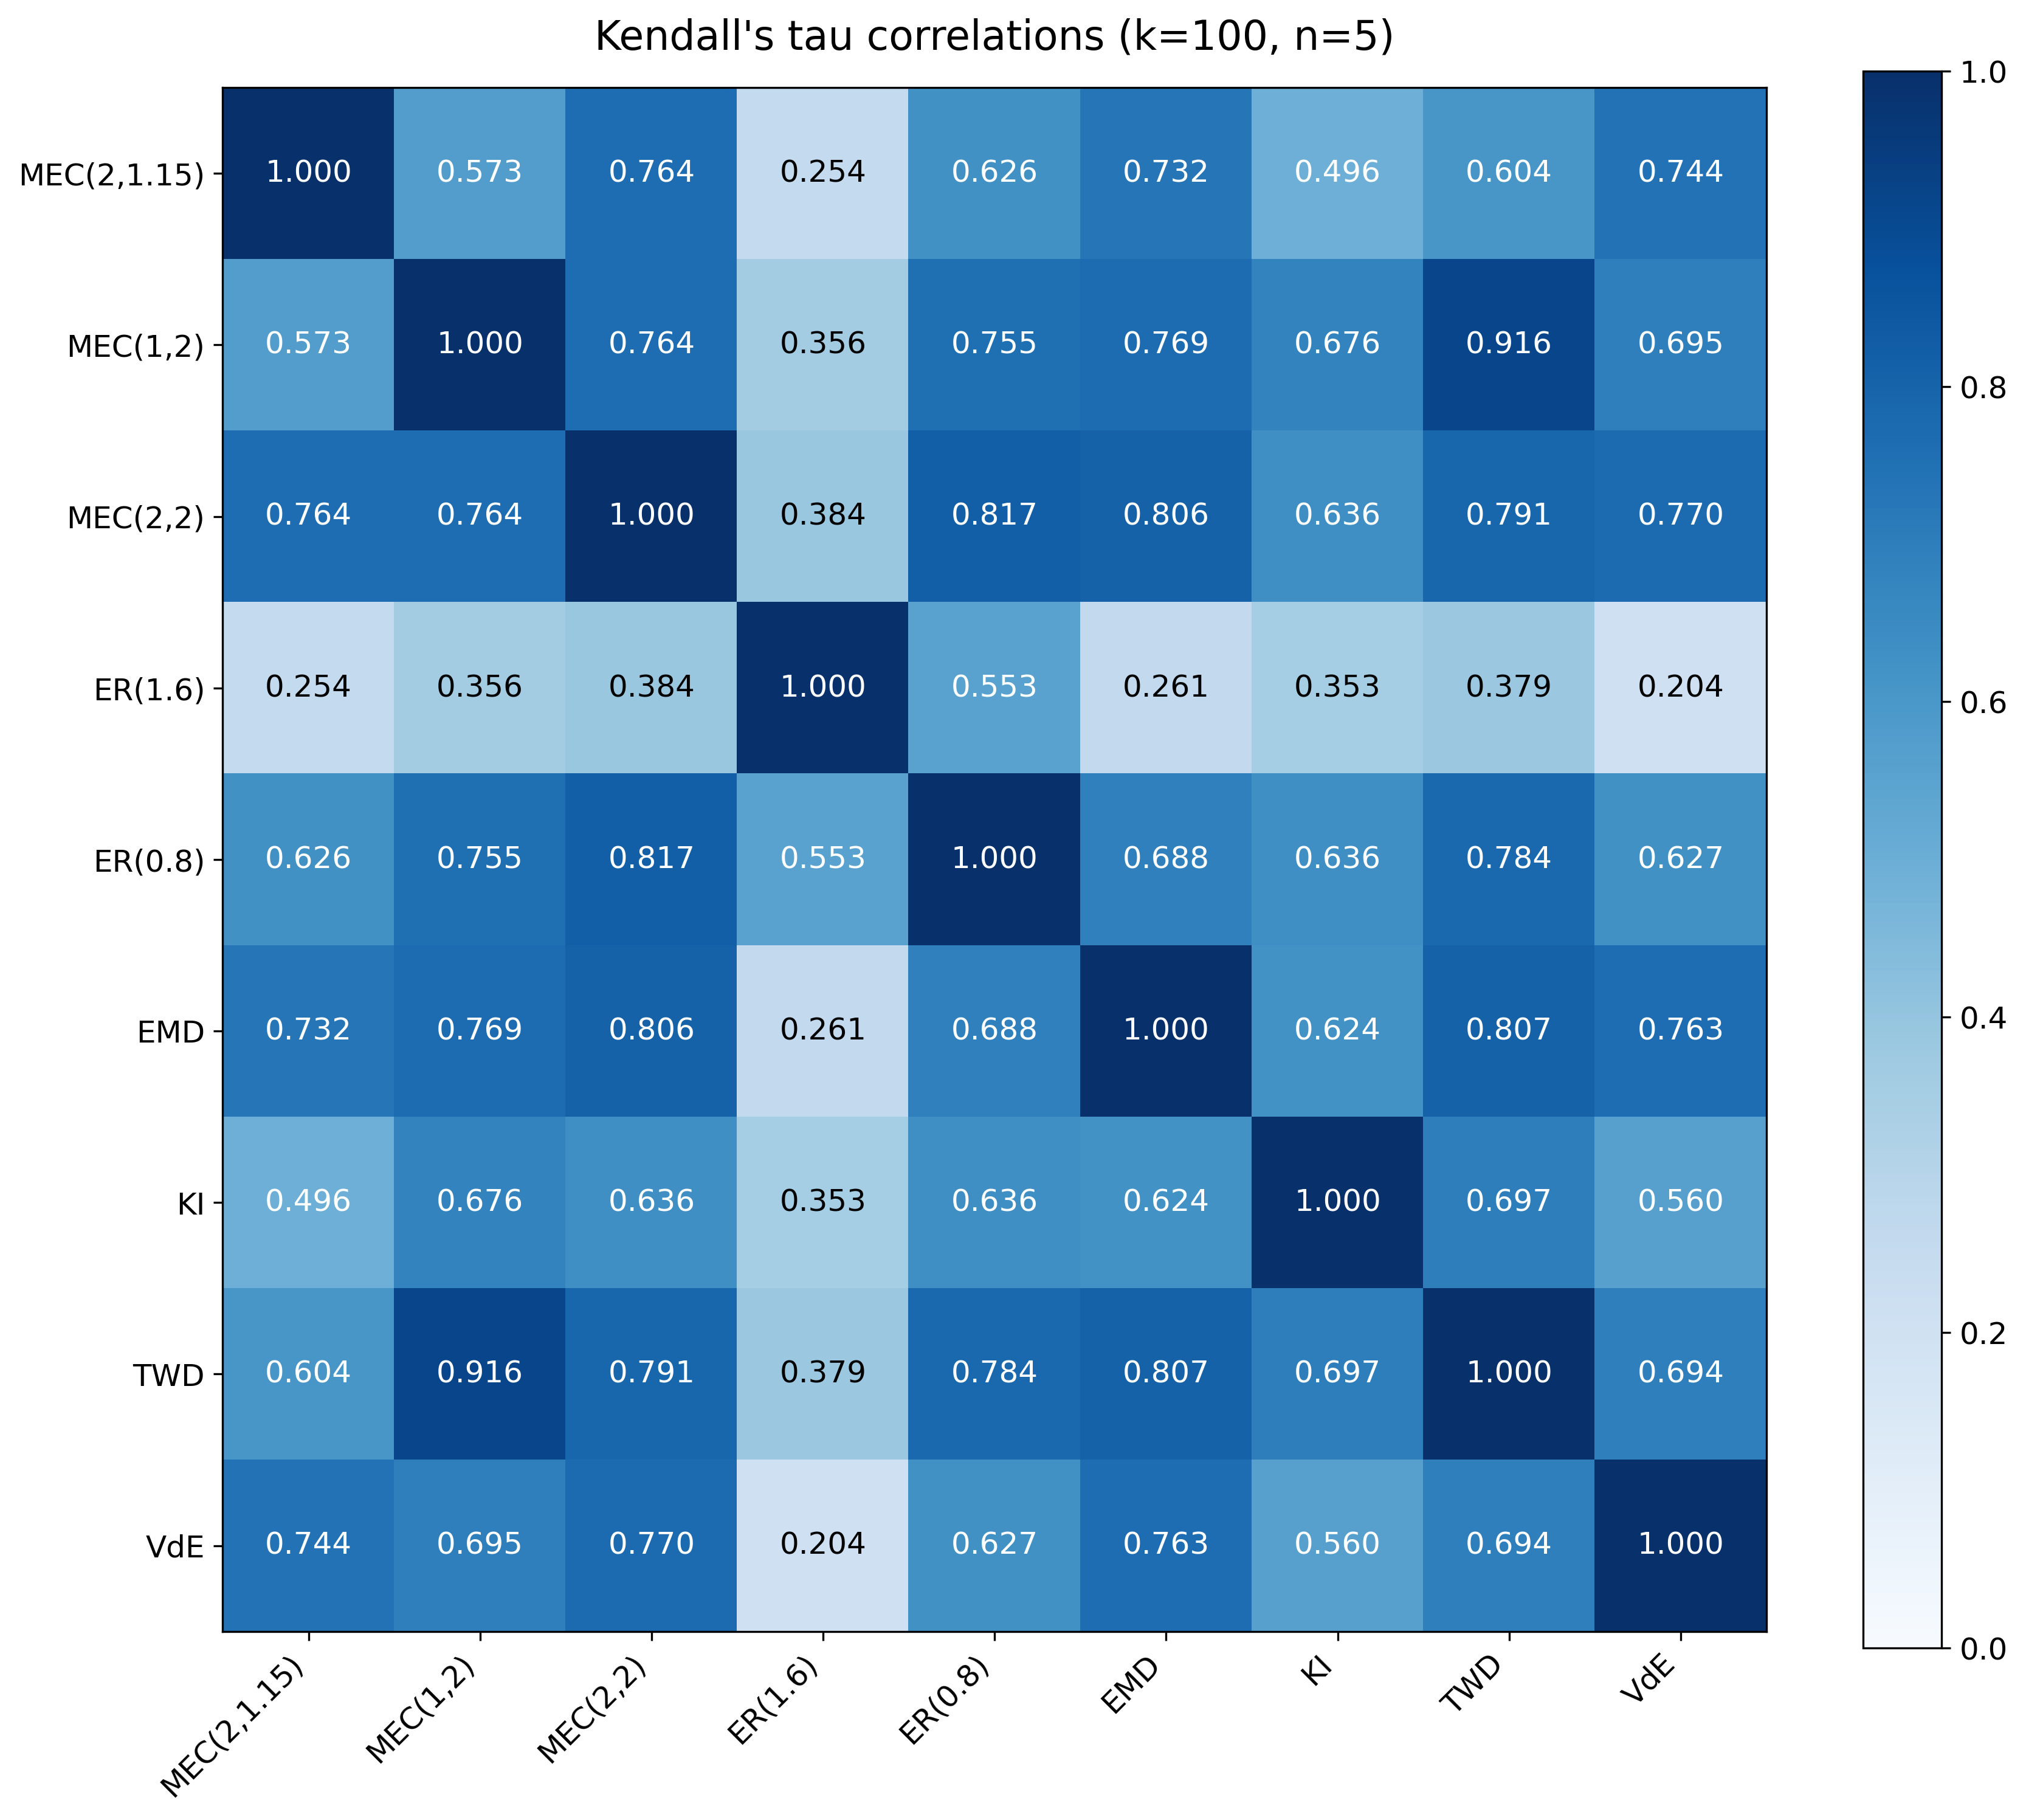
\includegraphics[width=0.78\linewidth]{Images/experimental_comparisons/kendalltau_correlation_matrix.png}
    \caption{Kendall's $\tau$ correlations among candidate polarization measures.}
    \label{fig:kendall-tau-correlation}
\end{figure}

Several interesting patterns emerge in the correlations. \TWDLabel{} shows particularly high agreement with $\MEC[1,2]$ ($\tau_B = 0.916$). This is consistent with their underlying structures: by Cor.~\ref{cor:mec-special-cases}, $\MEC[1,2]$ is the variance of $\bar\pi$ scaled by total mass, and \TWDLabel{} aggregates category probabilities weighted by distance from the mean opinion. Both are therefore mean-based dispersion measures, and the close empirical agreement reflects this shared structure rather than a coincidence between unrelated constructions. Conversely, \ERLabel[1.6]{} displays weak alignment with other indices ($\tau_B < 0.4$ in most cases), reflecting its distinctive emphasis on large-group identification effects under high $\alpha$. The value $\alpha=1.6$ is the upper bound $\alpha^*$ of the range $(0,\alpha^*]$ that Esteban and Ray~\cite{esteban1994measurement} prove admissible under their axioms (see Section~\ref{sec:er-axioms}). They note that larger $\alpha$ corresponds to greater \emph{polarization sensitivity}, i.e., a larger departure from inequality measurement.


\KILabel{} shows moderate correlations with most other indices (typically $0.5<\tau_B<0.7$), with the highest alignment to \TWDLabel{} ($\tau_B=0.697$). However, \KILabel{} has a significant theoretical limitation. By construction, it returns zero polarization whenever the population is absent from one side of the scale, i.e.\ whenever $\pi_1=\pi_2=0$ or $\pi_4=\pi_5=0$, even though distributions such as $(0,0,0.1,0.4,0.5)$ which clearly exhibits a non-consensus  structure. This illustrates the broader limitations of direct linear interpolation in capturing the complex structure of opinion polarization.

\subsection{Validation Against Expert Judgments}

Beyond the all-distribution analysis, we validated each polarization measure against expert judgment by replicating the experimental protocol introduced by Koudenburg, Kiers, and Kashima~\cite{koudenburg2021new}, where 60 researchers in polarization studies were asked to evaluate 15 hypothetical histograms, assigning each a score from 0 (not polarized) to 100 (maximally polarized). This ranking served as a human-derived baseline to evaluate how well each computational measure captures expert intuition. To quantify the alignment between each measure and expert judgment, we computed Kendall's $\tau_B$ between the expert ranking and the ordering induced by each measure across the 15 distributions.

\begin{figure}[H]
    \centering
    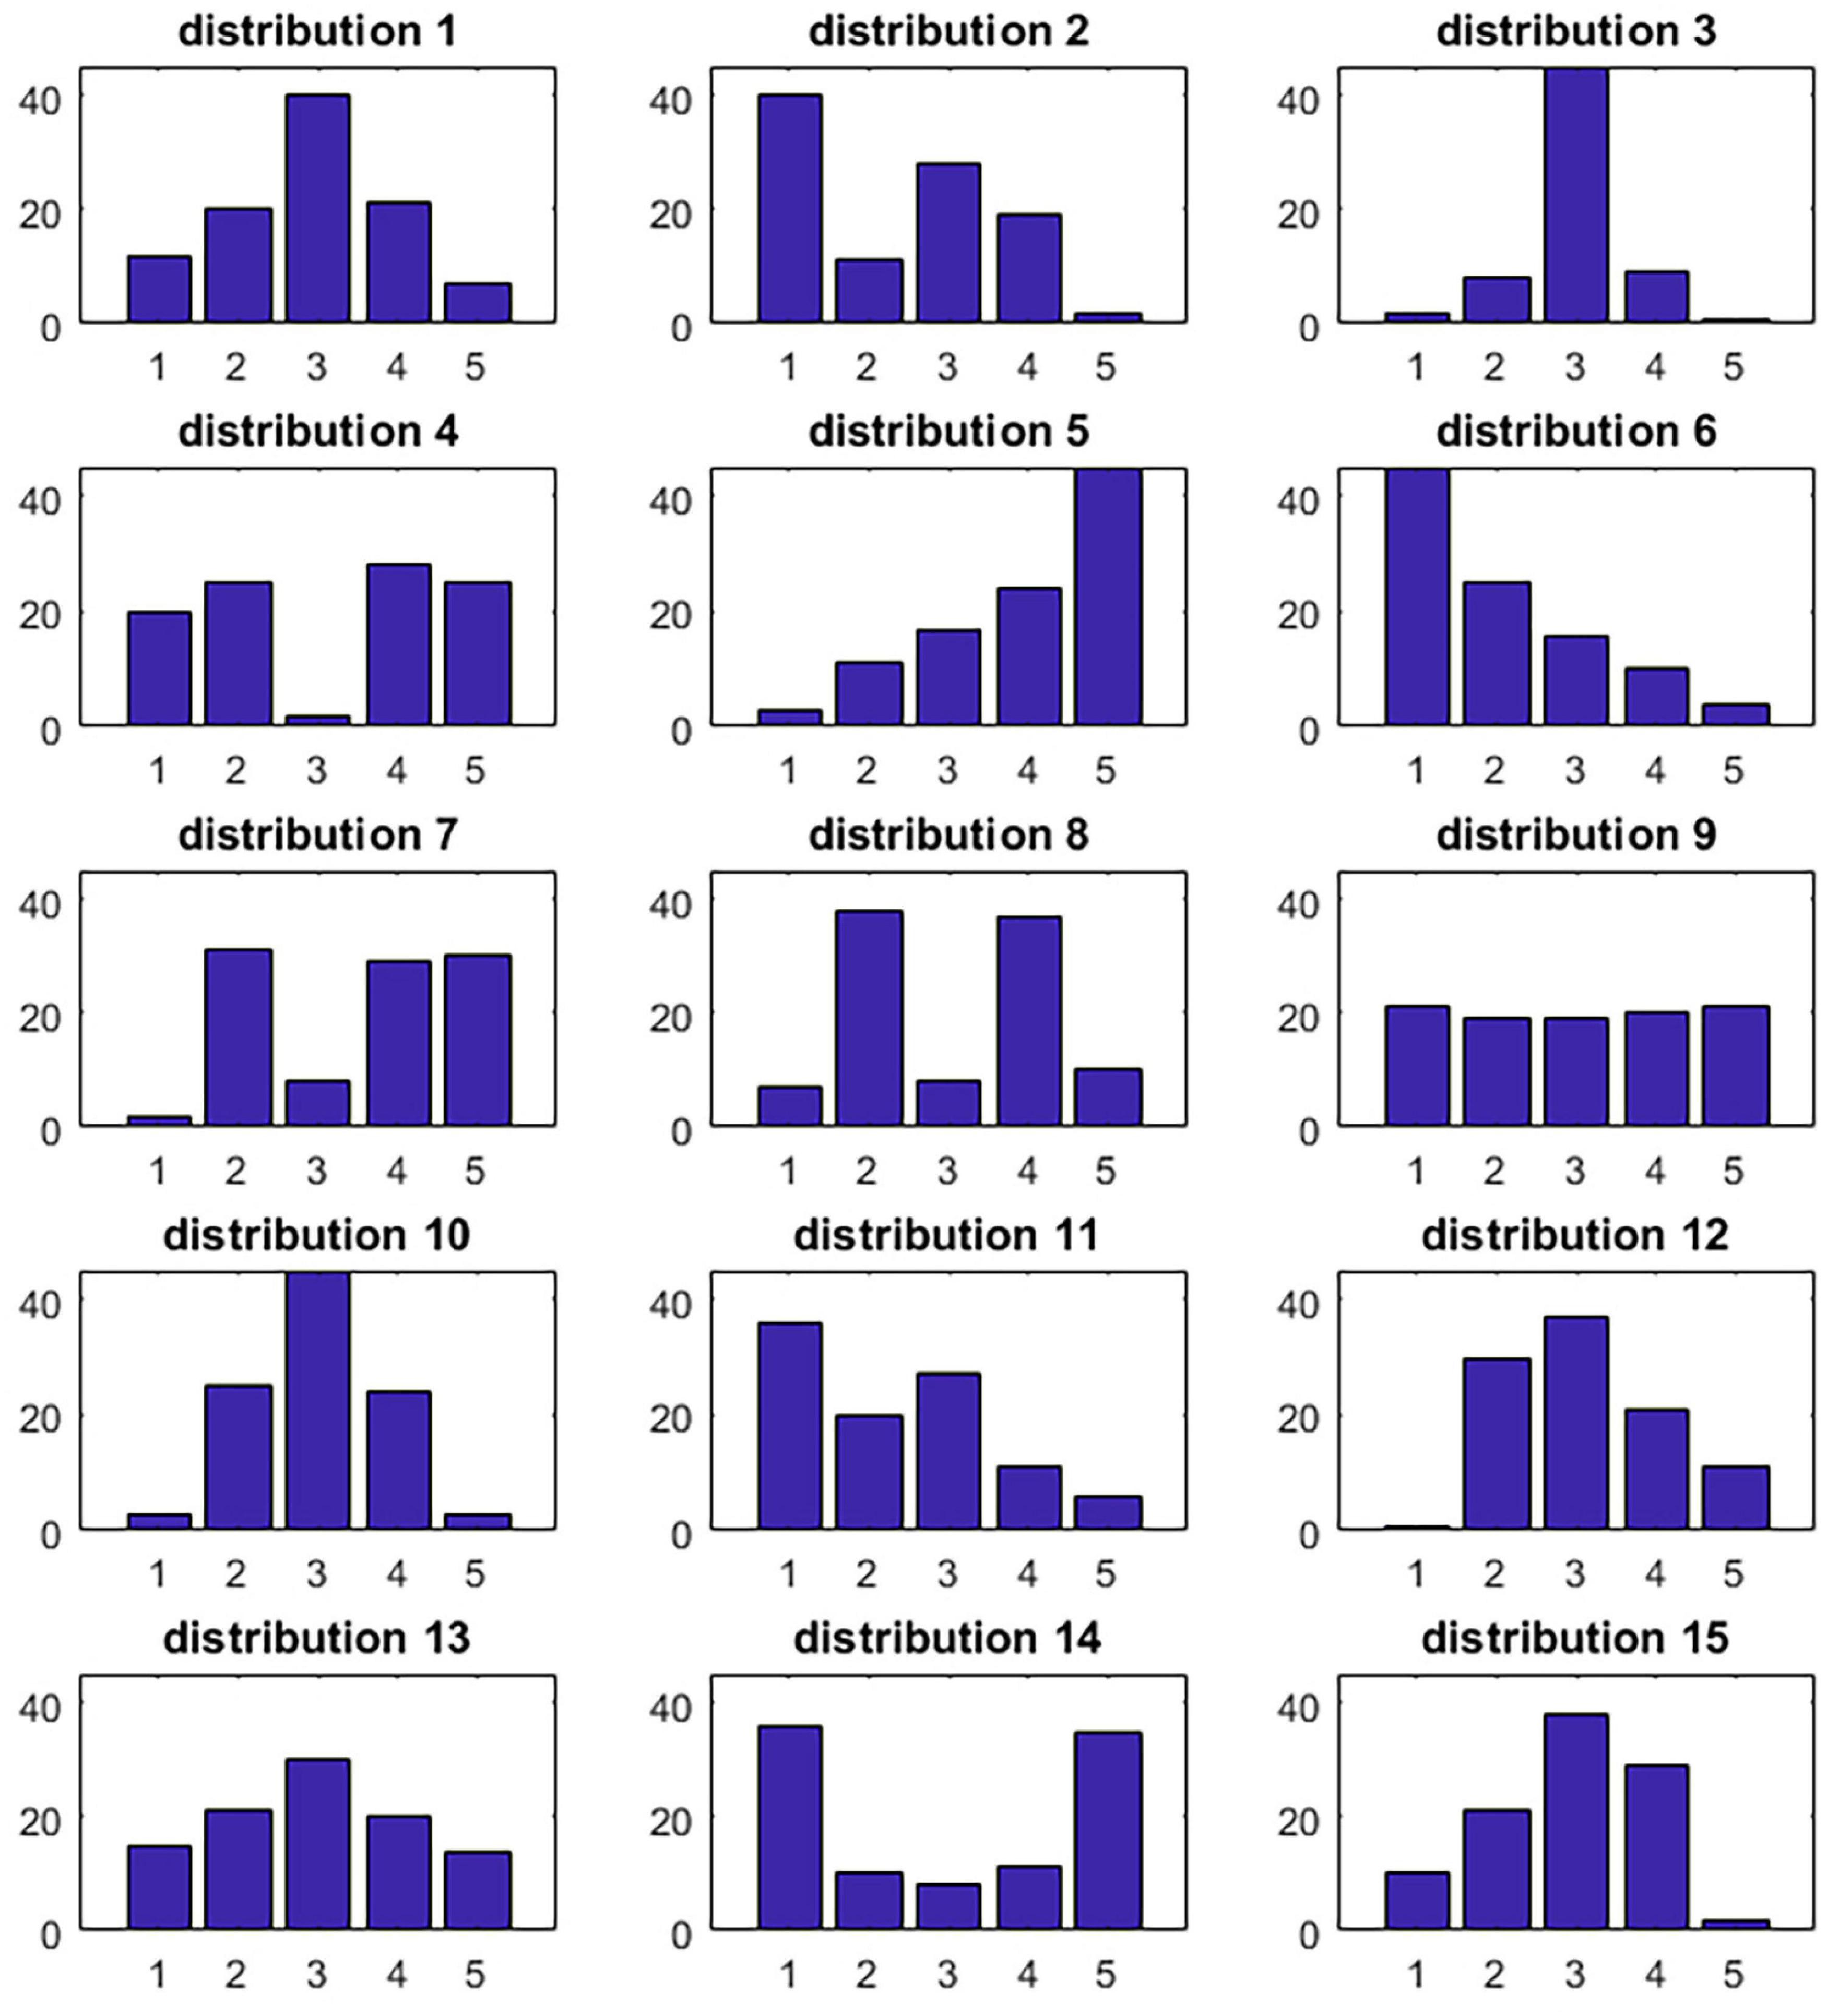
\includegraphics[width=0.6\linewidth]{Images/experimental_comparisons/experts_histograms.jpg}
    \caption{The 15 hypothetical distributions from \cite{koudenburg2021new} used for expert evaluation.}
    \label{fig:experts_histograms}
\end{figure}

\begin{figure}[H]
    \centering
    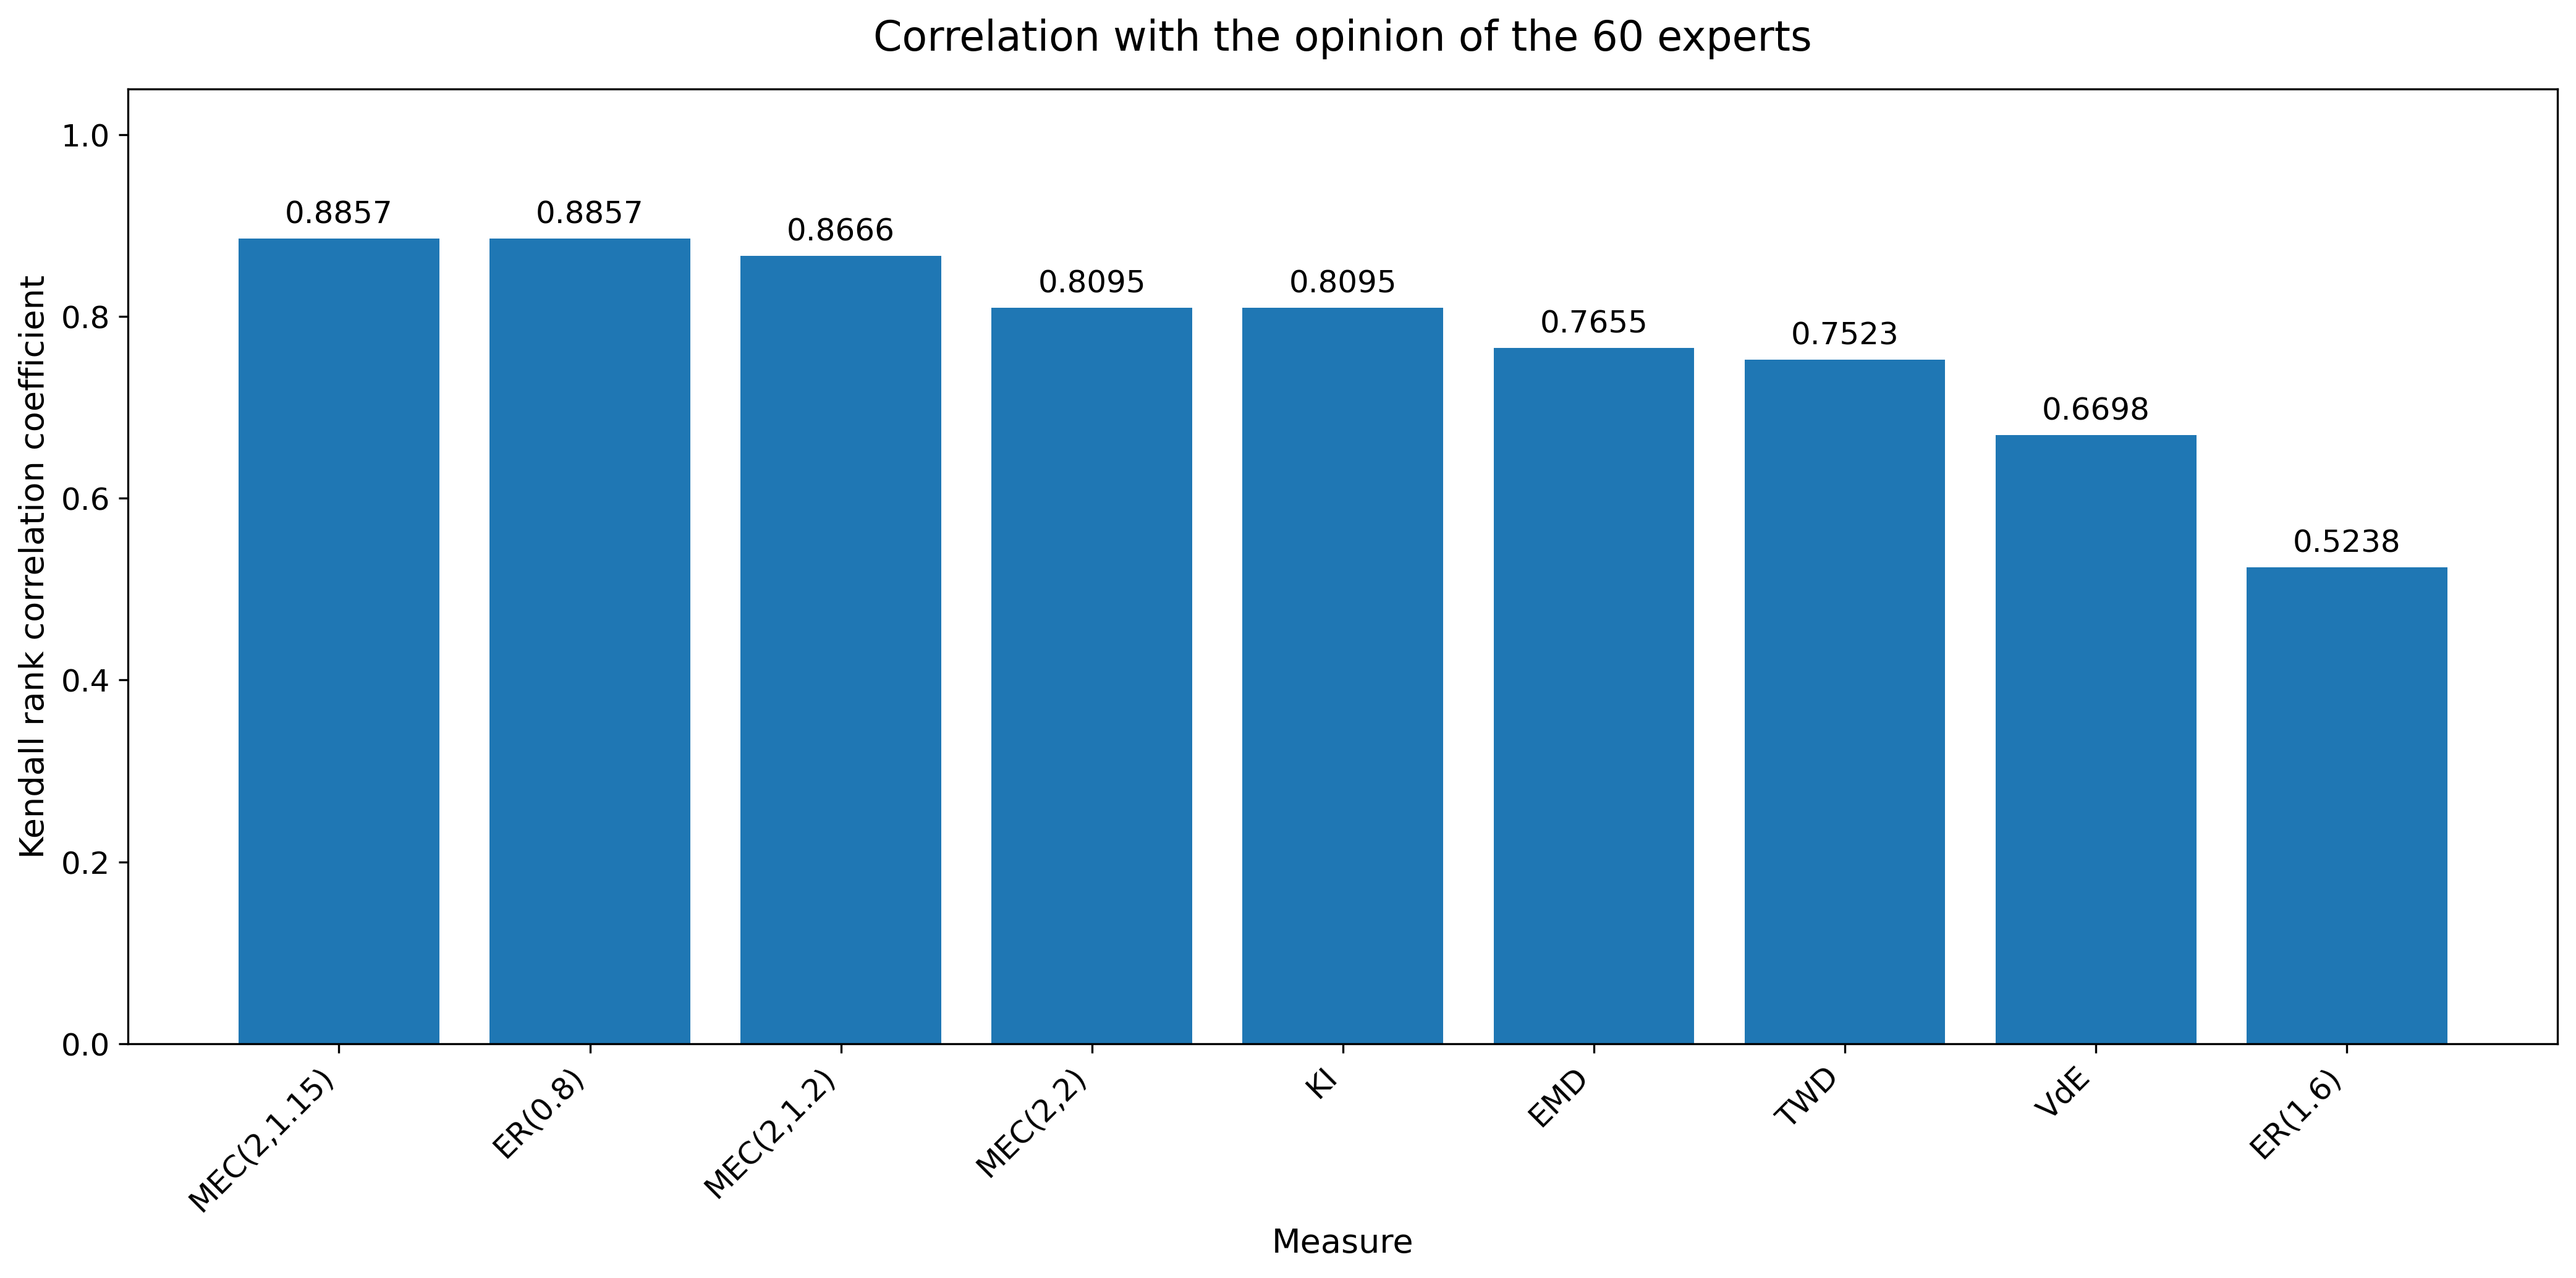
\includegraphics[width=0.85\linewidth]{Images/experimental_comparisons/correlation_experts_opinion.png}
    \caption{Correlation with expert judgments.}
    \label{fig:experts-opinion-correlation}
\end{figure}

The results highlight that $\MEC[2,1.15]$ and \ERLabel[0.8]{} show the highest concordance with expert evaluations, both achieving $\tau_{B}\approx 0.89$, whereas $\MEC[1,1]$ achieves $\tau_{B}=0.77$. In contrast, \VdELabel{} and \ERLabel[1.6]{} register lower correlations ($\tau_{B}=0.67$ and $\tau_{B}=0.52$, respectively). This divergence suggests that empirical agreement with expert judgments depends not only on broad normative motivation, but also on functional form, parameterization, and sensitivity to specific distributional patterns. This reinforces the need to complement axiomatic analysis with exhaustive empirical validation.
